% --- SLIDE 1: Einstein's Realism ---
\begin{frame}{The Clash of Titans: Einstein's Realism}

  \begin{columns}
    % Column for text
    \begin{column}{0.5\textwidth}
      \begin{itemize}[<+->] % Items appear one by one
        \item \textbf{Deterministic View:} The universe is knowable and orderly.
        \item \textbf{Objective Reality:} Physical properties exist independently of measurement.
        \item \textbf{No Fundamental Randomness:} Probability is not intrinsic to nature.
      \end{itemize}
    \end{column}

    % Column for image
    \begin{column}{0.5\textwidth}
      \begin{center}
        \begin{figure}
          \centering
          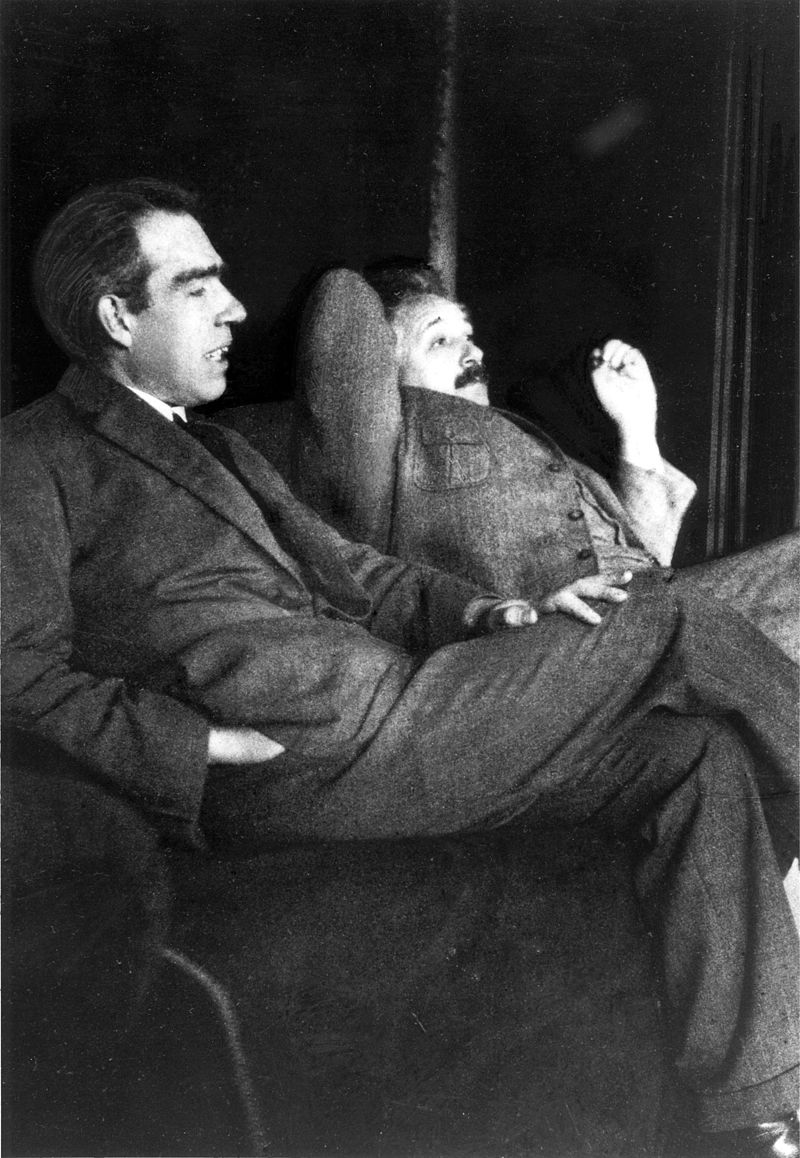
\includegraphics[width=0.5\linewidth]{images/Borhn-Einstein.jpg}
          \caption{Niels Bohr with Albert Einstein at Paul Ehrenfest's home in Leiden \cite{ehrenfest_niels_1925}.}
        \end{figure}
      \end{center}
    \end{column}
  \end{columns}

\end{frame}

% --- SLIDE 2: The EPR Paradox ---
\begin{frame}{The EPR Paradox: A Challenge in 1935}

  \begin{columns}
    % Column for text
    \begin{column}{0.55\textwidth} % Wider for the paper's text
      \begin{block}{The Seminal Paper}
        \begin{itemize}[<+->]
          \item In 1935, Einstein, Podolsky, and Rosen published a key paper.
          \item A ``frontal assault'' on the conceptual foundations of quantum mechanics.
          \item Their goal: To question whether the quantum description of reality is \emph{complete}.
          \item The title: ``Can Quantum-Mechanical Description of Physical Reality Be Considered Complete?''.
        \end{itemize}
      \end{block}
    \end{column}

    % Column for image
    \begin{column}{0.45\textwidth} % Narrower for the image
      \begin{center}
       \begin{figure}
        \centering
        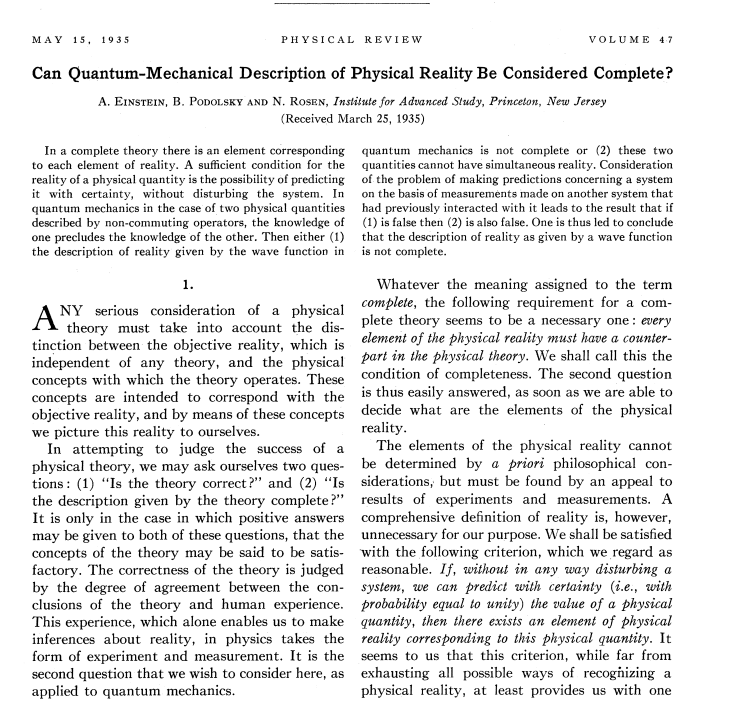
\includegraphics[width=0.5\linewidth]{images/EPR-articulo.png}
        \caption{Paper: Can Quantum-Mechanical Description of Physical Reality Be Considered Complete? \cite{einstein_can_1935}}
      \end{figure}
      \end{center}
    \end{column}
  \end{columns}

\end{frame}

% --- SLIDE 3: EPR's Criterion of Reality ---
\begin{frame}{The EPR Criterion of Reality}

  \begin{block}{The ``rule'' to define an element of reality}
    To formalize their attack, EPR introduced an explicit and, seemingly, irrefutable criterion:
  \end{block}
  \pause % Wait for a click to show the quote

  \begin{quote}
    ``If, without in any way disturbing a system, we can predict with certainty (i.e., with probability equal to unity) the value of a physical quantity, then there exists an element of physical reality corresponding to this physical quantity.''
  \end{quote}

\end{frame}

% --- SLIDE 4: Violation of the Criterion ---
\begin{frame}{Violation of the Criterion: Position and Momentum}

  \begin{block}{Example with a state $\psi = e^{(2\pi i/h)p_0x}$}
    \begin{itemize}[<+->] % Items appear one by one
      \item When applying the momentum operator ($p$), we get an exact value:
      $$ p\psi = \left(\frac{h}{2\pi i}\frac{\partial}{\partial x}\right)\psi = p_0\psi $$
      It is concluded that the momentum, $p_0$, is an \textbf{element of reality}.
      \item However, when applying the position operator ($x$), an exact value is not obtained:
      $$ x\psi \neq \text{constant} \cdot \psi $$
      We can only calculate the \textbf{probability} of finding the particle in an interval $[a, b]$, which turns out to be $P(a,b) = b-a$.
    \end{itemize}
  \end{block}

\end{frame}

% --- SLIDE 5: The EPR Conclusion ---
\begin{frame}{The EPR Conclusion}

  \begin{alertblock}{The Fundamental Dichotomy}
    From the previous example, it follows that there are only two possibilities:
    \begin{enumerate}[<+->] % List items appear one by one
        \item Either the quantum-mechanical description of reality given by the wave function \textbf{is not complete}.
        \item Or when the operators for two physical quantities do not commute, the two quantities \textbf{cannot have simultaneous reality}.
    \end{enumerate}
  \end{alertblock}
\end{frame}

% --- SLIDE 6: The Principle of Locality ---
\begin{frame}{The Principle of Locality}

  \begin{block}{A fundamental idea in physics}
    \begin{itemize}[<+->] % Items appear one by one
      \item An object can only be directly influenced by its \textbf{immediate surroundings}.
      \item Any influence at a distance cannot be instantaneous; it must propagate at a finite speed, not exceeding the speed of light ($c$).
      \item For Einstein, locality was a sacred axiom. Its violation would imply the disintegration of the universe's \textbf{causal structure} (cause-and-effect).
    \end{itemize}
  \end{block}

\end{frame}

% --- SLIDE 7: The EPR Thought Experiment ---
\begin{frame}{The EPR Thought Experiment}

  \begin{columns}[T] % Align columns at the top
    % Column for text
    \begin{column}{0.6\textwidth}
      \begin{block}{The two-particle system}
        \begin{itemize}[<+->]
          \item A system of two particles is prepared in an entangled state and then separated by a large distance.
          \item \textbf{Option 1:} If Alice measures the \textbf{momentum} of her particle, she can predict with certainty the momentum of Bob's particle.
          \item \textbf{Option 2:} If Alice measures the \textbf{position}, she can predict with certainty Bob's position.
          \item \textbf{Partial Conclusion:} Both the position and momentum of Bob's particle must be ``elements of reality''.
        \end{itemize}
      \end{block}
    \end{column}

    % Column for image
    \begin{column}{0.4\textwidth}
      \begin{figure}
        \centering
        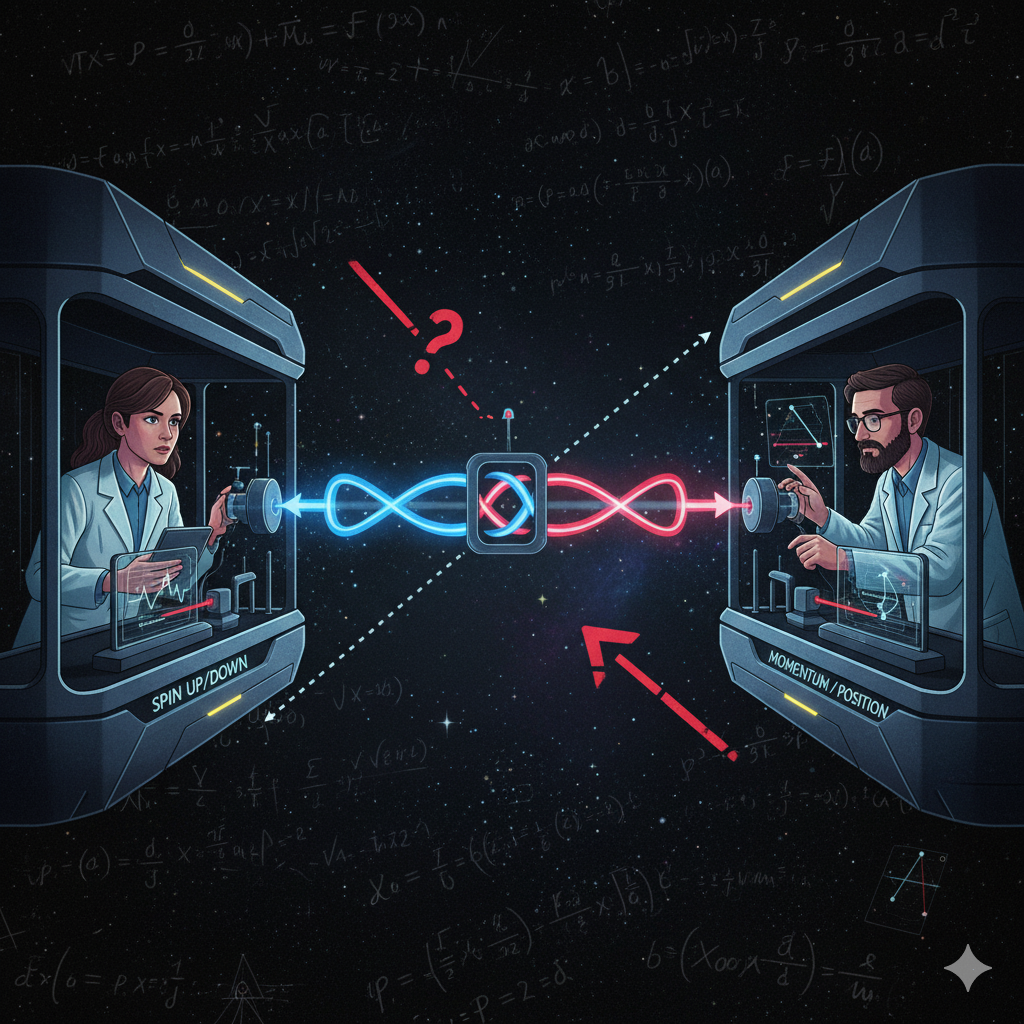
\includegraphics[width=\linewidth]{images/epr_experiment.png}
        \caption{Alice and Bob measure entangled particles separated by a large distance \cite{googlo_ilustracion_2025}.}
      \end{figure}
    \end{column}
  \end{columns}

\end{frame}

% --- SLIDE 8: The Contradiction and EPR's Conclusion ---
\begin{frame}{The Contradiction and EPR's Conclusion}

  \begin{block}{The Conflict with Quantum Mechanics}
    \begin{itemize}[<+->]
      \item The conclusion that Bob's particle has a definite position and momentum \textbf{simultaneously}...
      \item ...is in direct conflict with the \textbf{Heisenberg Uncertainty Principle}, which forbids it.
    \end{itemize}
  \end{block}

  \begin{alertblock}<3->{The EPR Conclusion}
    Faced with this dilemma, if local realism is correct, the only possible conclusion is that:
    \begin{itemize}[<+->]
      \item The description of reality provided by the wave function must be \textbf{incomplete}.
      \item There must be an underlying theory (``hidden variables'') that provides a complete description.
    \end{itemize}
  \end{alertblock}

\end{frame}

% --- SLIDE 9: Bohr's Response ---
\begin{frame}{Bohr's Response: The Principle of Complementarity}

  \begin{columns}[T] % Align columns at the top
    % Column for text
    \begin{column}{0.55\textwidth}
      \begin{block}{Mutually Exclusive, Yet Necessary Concepts}
        \begin{itemize}[<+->] % Items appear one by one
          \item Complementarity posits that pairs of classical concepts are necessary for a complete description.
          \item But they are \textbf{mutually exclusive} in any single experiment.
          \item They are not contradictory properties of the object, but complementary aspects of a \textbf{phenomenon} revealed by incompatible experimental arrangements.
        \end{itemize}
    \end{block}
    \end{column}

    % Column for image
    \begin{column}{0.45\textwidth}
      \begin{figure}
        \centering
        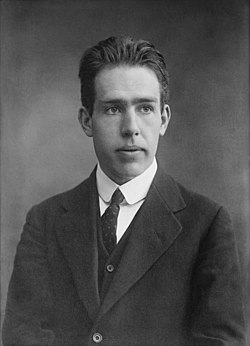
\includegraphics[width=\linewidth, height=0.7\textheight, keepaspectratio]{images/NielsBohr.jpg}
        \caption{Niels Bohr \cite{bain_news_service_prof_1910}.}
      \end{figure}
    \end{column}
  \end{columns}

\end{frame}

% --- SLIDE 10: Is Quantum Mechanics Complete? Bohr's View ---
\begin{frame}{Is Quantum Mechanics Complete? Bohr's View}

  \begin{block}{Radical Revision of Physical Reality}
    \begin{itemize}[<+->]
      \item The experimenter's ``freedom of choice'' does not reveal pre-existing realities, but rather \textbf{creates different experimental conditions} and phenomena.
      \item Quantum mechanics is \textbf{complete} because it correctly and exhaustively describes the results of \emph{every possible, well-defined experiment}.
      \item Bohr compares this revision of physical reality to the modification of ideas about the absolute character of phenomena introduced by the \textbf{Theory of Relativity}.
      \item This philosophical debate was crucial and led to \textbf{Bell's Theorem} and subsequent experiments, turning EPR into a testable question.
    \end{itemize}
  \end{block}

\end{frame}

% --- SLIDE 11: Schrödinger's Response ---
\begin{frame}{Schrödinger's Response: The Birth of ``Entanglement''}

  \begin{columns}[T] % Align columns at the top
    % Column for text
    \begin{column}{0.6\textwidth}
      \begin{block}{Context and the Essence of the New Physics}
        \begin{itemize}[<+->]
          \item A few months after EPR, Schrödinger published his response: ``Discussion of Probability Relations between Separated Systems''.
          \item He demonstrated a deep understanding and took the EPR argument to its most extreme conclusions.
          \item He understood that the phenomenon was not an anomaly, but \textbf{the characteristic trait of quantum mechanics}.
          \item He coined the term \textbf{``Entanglement'' (Verschränkung)}.
        \end{itemize}
    \end{block}
\end{column}

    % Column for image
    \begin{column}{0.4\textwidth}
      \begin{figure}
        \centering
        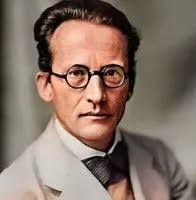
\includegraphics[width=\linewidth, height=0.7\textheight, keepaspectratio]{images/schrodinger.jpeg}
        \caption{Erwin Schrödinger \cite{fotografo_desconocido_retrato_1933}.}
      \end{figure}
    \end{column}
  \end{columns}

\end{frame}

% --- SLIDE 12: Steering ---
\begin{frame}{``Steering'' and the Schmidt Decomposition}

  \begin{block}{The most unsettling aspect of Entanglement}
    \begin{itemize}[<+->]
      \item Schrödinger identified an experimenter's ability to \textbf{``steer'' (steuern)} the state of a distant system.
      \item This is achieved through the local choice of measurement.
      \item He described it as ``rather discomforting that the theory allows a system to be steered... at the whim of the experimenter, even though they have no access to it''.
      \item Rigorously demonstrated with a mathematical formalism: the \textbf{Schmidt decomposition}.
    \end{itemize}
  \end{block}

\end{frame}

% --- SLIDE 13: Bohr vs. Schrödinger ---
\begin{frame}{Bohr vs. Schrödinger: Two Approaches to the Paradox}

  \begin{block}{Fundamental Differences in the Response to EPR}
    \begin{itemize}[<+->]
      \item \textbf{Bohr:} Offered a philosophical framework (complementarity) to \emph{dissolve the paradox}, declaring that EPR's questions were ill-posed.
      \item \textbf{Schrödinger:} Accepted the validity of EPR's questions and delved into the unsettling answers the theory provided, seeking to \emph{intensify the paradox}.
    \end{itemize}
  \end{block}

  \begin{alertblock}<3->{Schrödinger's Key Contributions}
    \begin{itemize}[<+->]
      \item \textbf{Named and defined the central concept:} He coined the term ``entanglement''.
      \item \textbf{Identified its most powerful manifestation:} The concept of ``steering,'' which captured the essence of non-locality.
      \item \textbf{Proved its generality with mathematical rigor:} He extended the EPR argument to all observables, showing its structural nature.
    \end{itemize}
  \end{alertblock}

\end{frame}
